%!TEX root = ../thesis.tex
%*******************************************************************************
%****************************** Third Chapter **********************************
%*******************************************************************************
\chapter{Discussion}

% **************************** Define Graphics Path **************************

\graphicspath{{Chapter5/Figs/Vector/}{Chapter5/Figs/}}


\section{Non-Parametric}
Three algorithms tested of non-parametric variety producing several noticeable results. Firstly, Monte Carlo sampling outperformed both Greedy and RoD sampling. This is demonstrated convincingly through Figure~\ref{fig:nPComp} where results from the greedy results suggest the worst accuracy.

Despite the greedy algorithm demonstrating the worst accuracy, interesting results were shown with ROD sampling. Poor selection is evidently present with the first sample set, although rapid improvement quickly follows. Indeed, after the first iteration, the learning rate is superior to the other two algorithms. An extra iteration may indeed have seen RoD surpassing Monte Carlo. This is expected as the ROD algorithm specifically targets regions of the model which are challenging causing the largest changes towards proper fitting.

Both ROD and greedy sampling are suspected to suffer from clusterisation whereby data points similar to each other in the feature space are sampled within the same batch, thus reducing the total information conveyed per batch operation. This is believed to be particularly costly with the first iteration as the model will heavily overfit to the new cluster it has sampled. The random nature of Monte Carlo reduces this prospect, hence the apparent promising performance of a random sampling methodology. Evidence to this is shown in Figure~\ref{fig:MCTestSet}, Figure~\ref{fig:GreedyTestSet}, and Figure~\ref{fig:RODTestSet}.

\begin{figure}[h]
    \begin{center}
        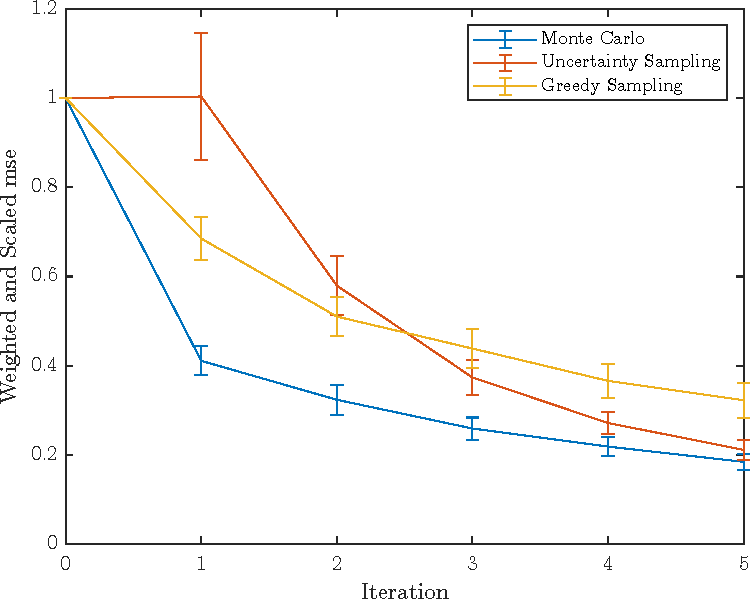
\includegraphics{nonParamComp1.pdf}
        \caption[Non-parametric comparison]{Comparison of different non-parametric algorithms with standard deviations represented as error bars.}
        \label{fig:nPComp}
    \end{center}
\end{figure}

This demonstrates a danger with Batch Active Learning. It is very easy to produce a learning algorithm which actually performs worse than random screening.

\section{Parametric}
Different classes of parametric algorithms were tested. The first of these is a first order composite algorithm, RoD with Greed: i.e. uses different active learning algorithms as a base. The second is a clustering algorithm with the number of clusters left as a parameter. The third is a second order composite active learning algorithm which combines the other two parametric functions, affectionately named the Holy Trinity. A constant improvement is seen throughout these algorithms, with the Holy Trinity performing the best.

\begin{figure}[h]
    \begin{center}
        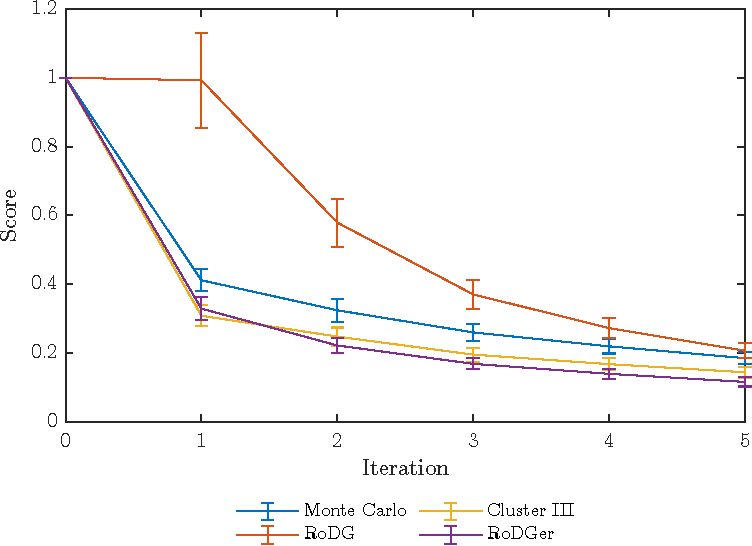
\includegraphics{paramComp1.pdf}
        \caption[Non-parametric comparison]{Comparison of different parametric algorithms with standard deviations represented as error bars.}
        \label{fig:pComp}
    \end{center}
\end{figure}

Several points of interest are highlighted with these results. Firstly, despite improving upon RoD, RoD with Greed is still beaten by Monte Carlo sampling. Again, the methodology suffers from clustering of points. This is shown with the ability of Cluster III outperforming Monte Carlo. The progression through the different cluster algorithms also sees improvement with progression, as anticipated.

The sampling process of the Cluster III algorithm demonstrates its ability at outperforming the random sampling methodology of Monte Carlo even within the first iteration. The Holy Trinity algorithm sacrifices some of this initial performance for longer term gain, as shown by the worse performance after the first iteration. By the second iteration, the difference becomes insignificant, with the error for each algorithm. By the end of the fifth iteration, the Holy Trinity algorithm convincingly outperforms the other algorithms.

Upon investigation of the parameters settled upon within these several points arise. Firstly with RoD with Greed, at low $\alpha$, WMSE appears uncorrelated with $\alpha$, only experiencing a significant rise with $\alpha{}>0.4$. Thus, it can be surmised that RoD is the driving force, with evidence given by the final scores for RoD and RoD with Greed algorithms arising within error of each other.

On the other hand, the sensitivity of Cluster III is extremely low to cluster size, demonstrated by Figure~\ref{fig:clusterTest}. Here, no significant change is observed within the significant parameter range. It is believed this is due to highest ranking points remaining within the top clusters as large clusters are likely to remain the largest, even with an increased number of clusters. Thus, the top candidates are likely to remain in the same region of the feature space.